\section{\huge Analisi degli Utenti}
L'analisi degli utenti per \textbf{DressCode} identifica i principali utilizzatori di \textbf{DressCode}, un costruttore di moduli web progettato per semplicità e personalizzazione con un tema abbigliamento. Tre gruppi emergono come target primari: sviluppatori web, designer grafici e piccole imprese (PMI).
\\\\
Gli sviluppatori web, spesso freelance o parte di team agili, cercano uno strumento rapido per creare moduli integrabili nei loro siti, valorizzando funzionalità come l'esportazione in HTML/JavaScript e l'editor avanzato. I designer grafici, abituati a strumenti visivi come Figma, apprezzano l'interfaccia intuitiva e la personalizzazione estetica (es. temi Accessori), ma potrebbero richiedere schemi predefiniti accattivanti. Le PMI, con competenze tecniche limitate, necessitano di un sistema facile da usare per moduli di contatto o sondaggi, privilegiando usabilità e pubblicazione diretta nella Vetrina.
\\\\
Questi utenti condividono l'esigenza di un'esperienza semplice e distintiva, che \textbf{DressCode} soddisfa con il suo approccio tematico e l'integrazione fluida. La sfida sarà bilanciare la semplicità per le PMI con le opzioni avanzate per sviluppatori e designer, testando il prototipo con ciascun gruppo.
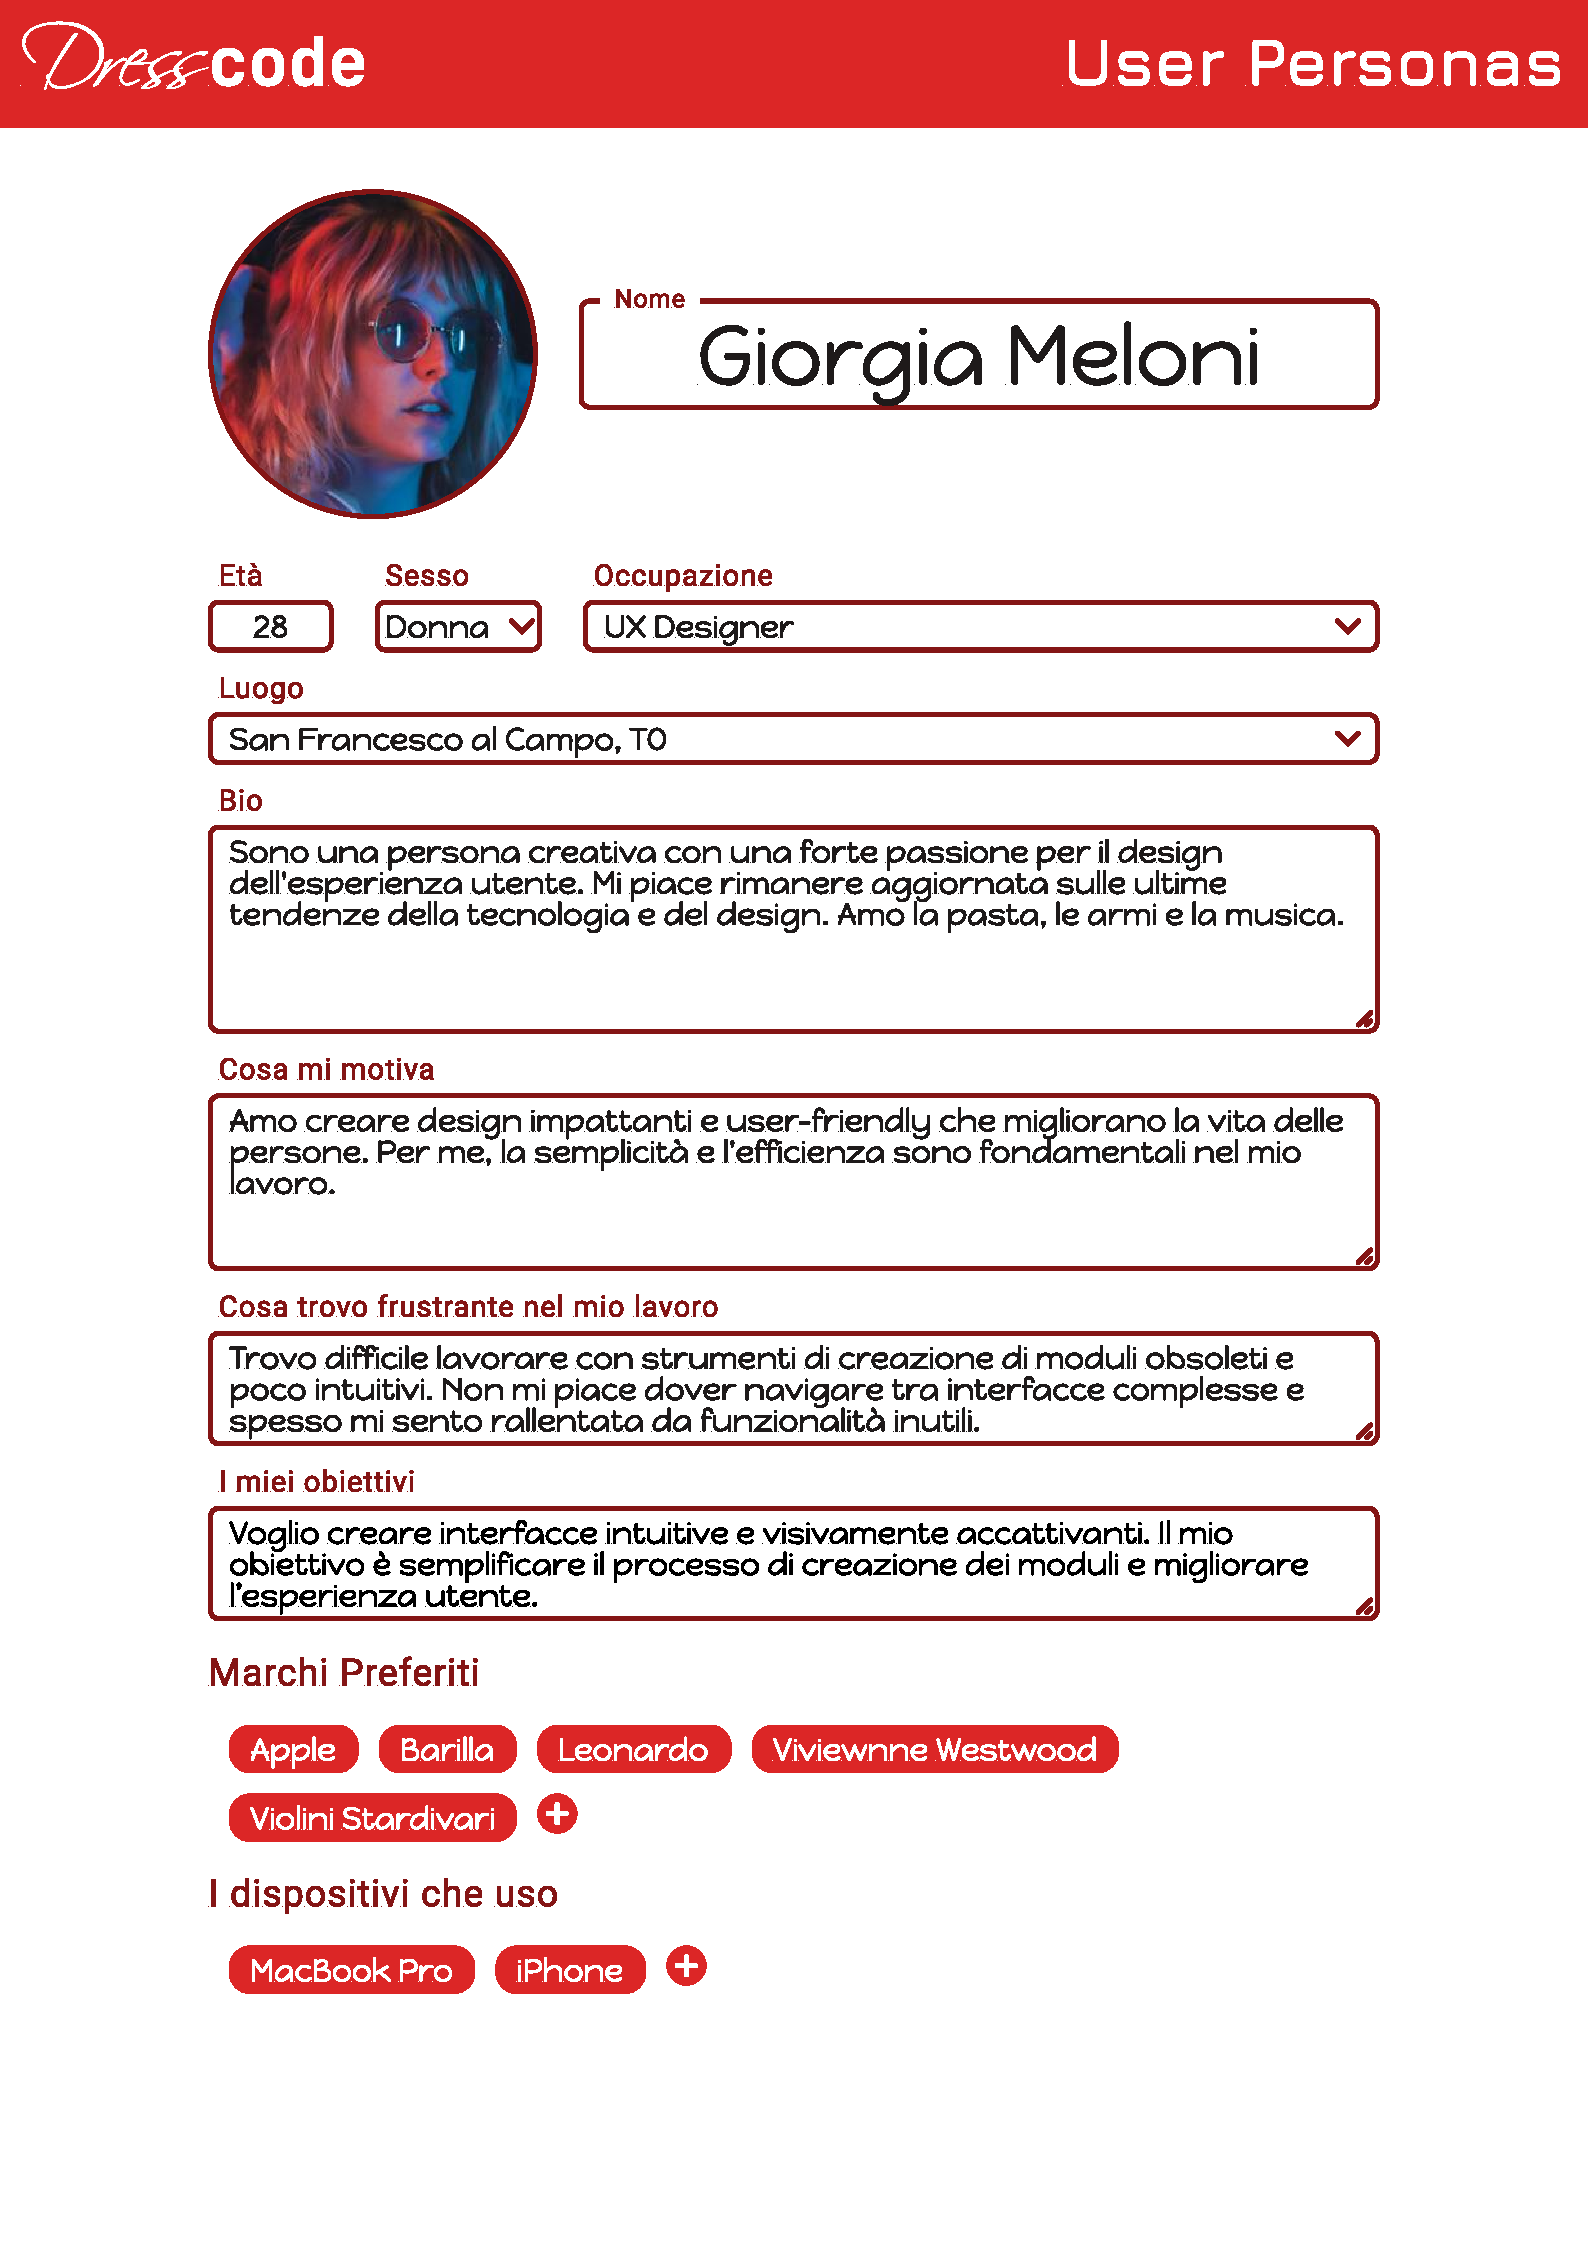
\includepdf[pages=-,pagecommand={}]{analisi degli utenti/personas_giorgia_meloni.pdf}
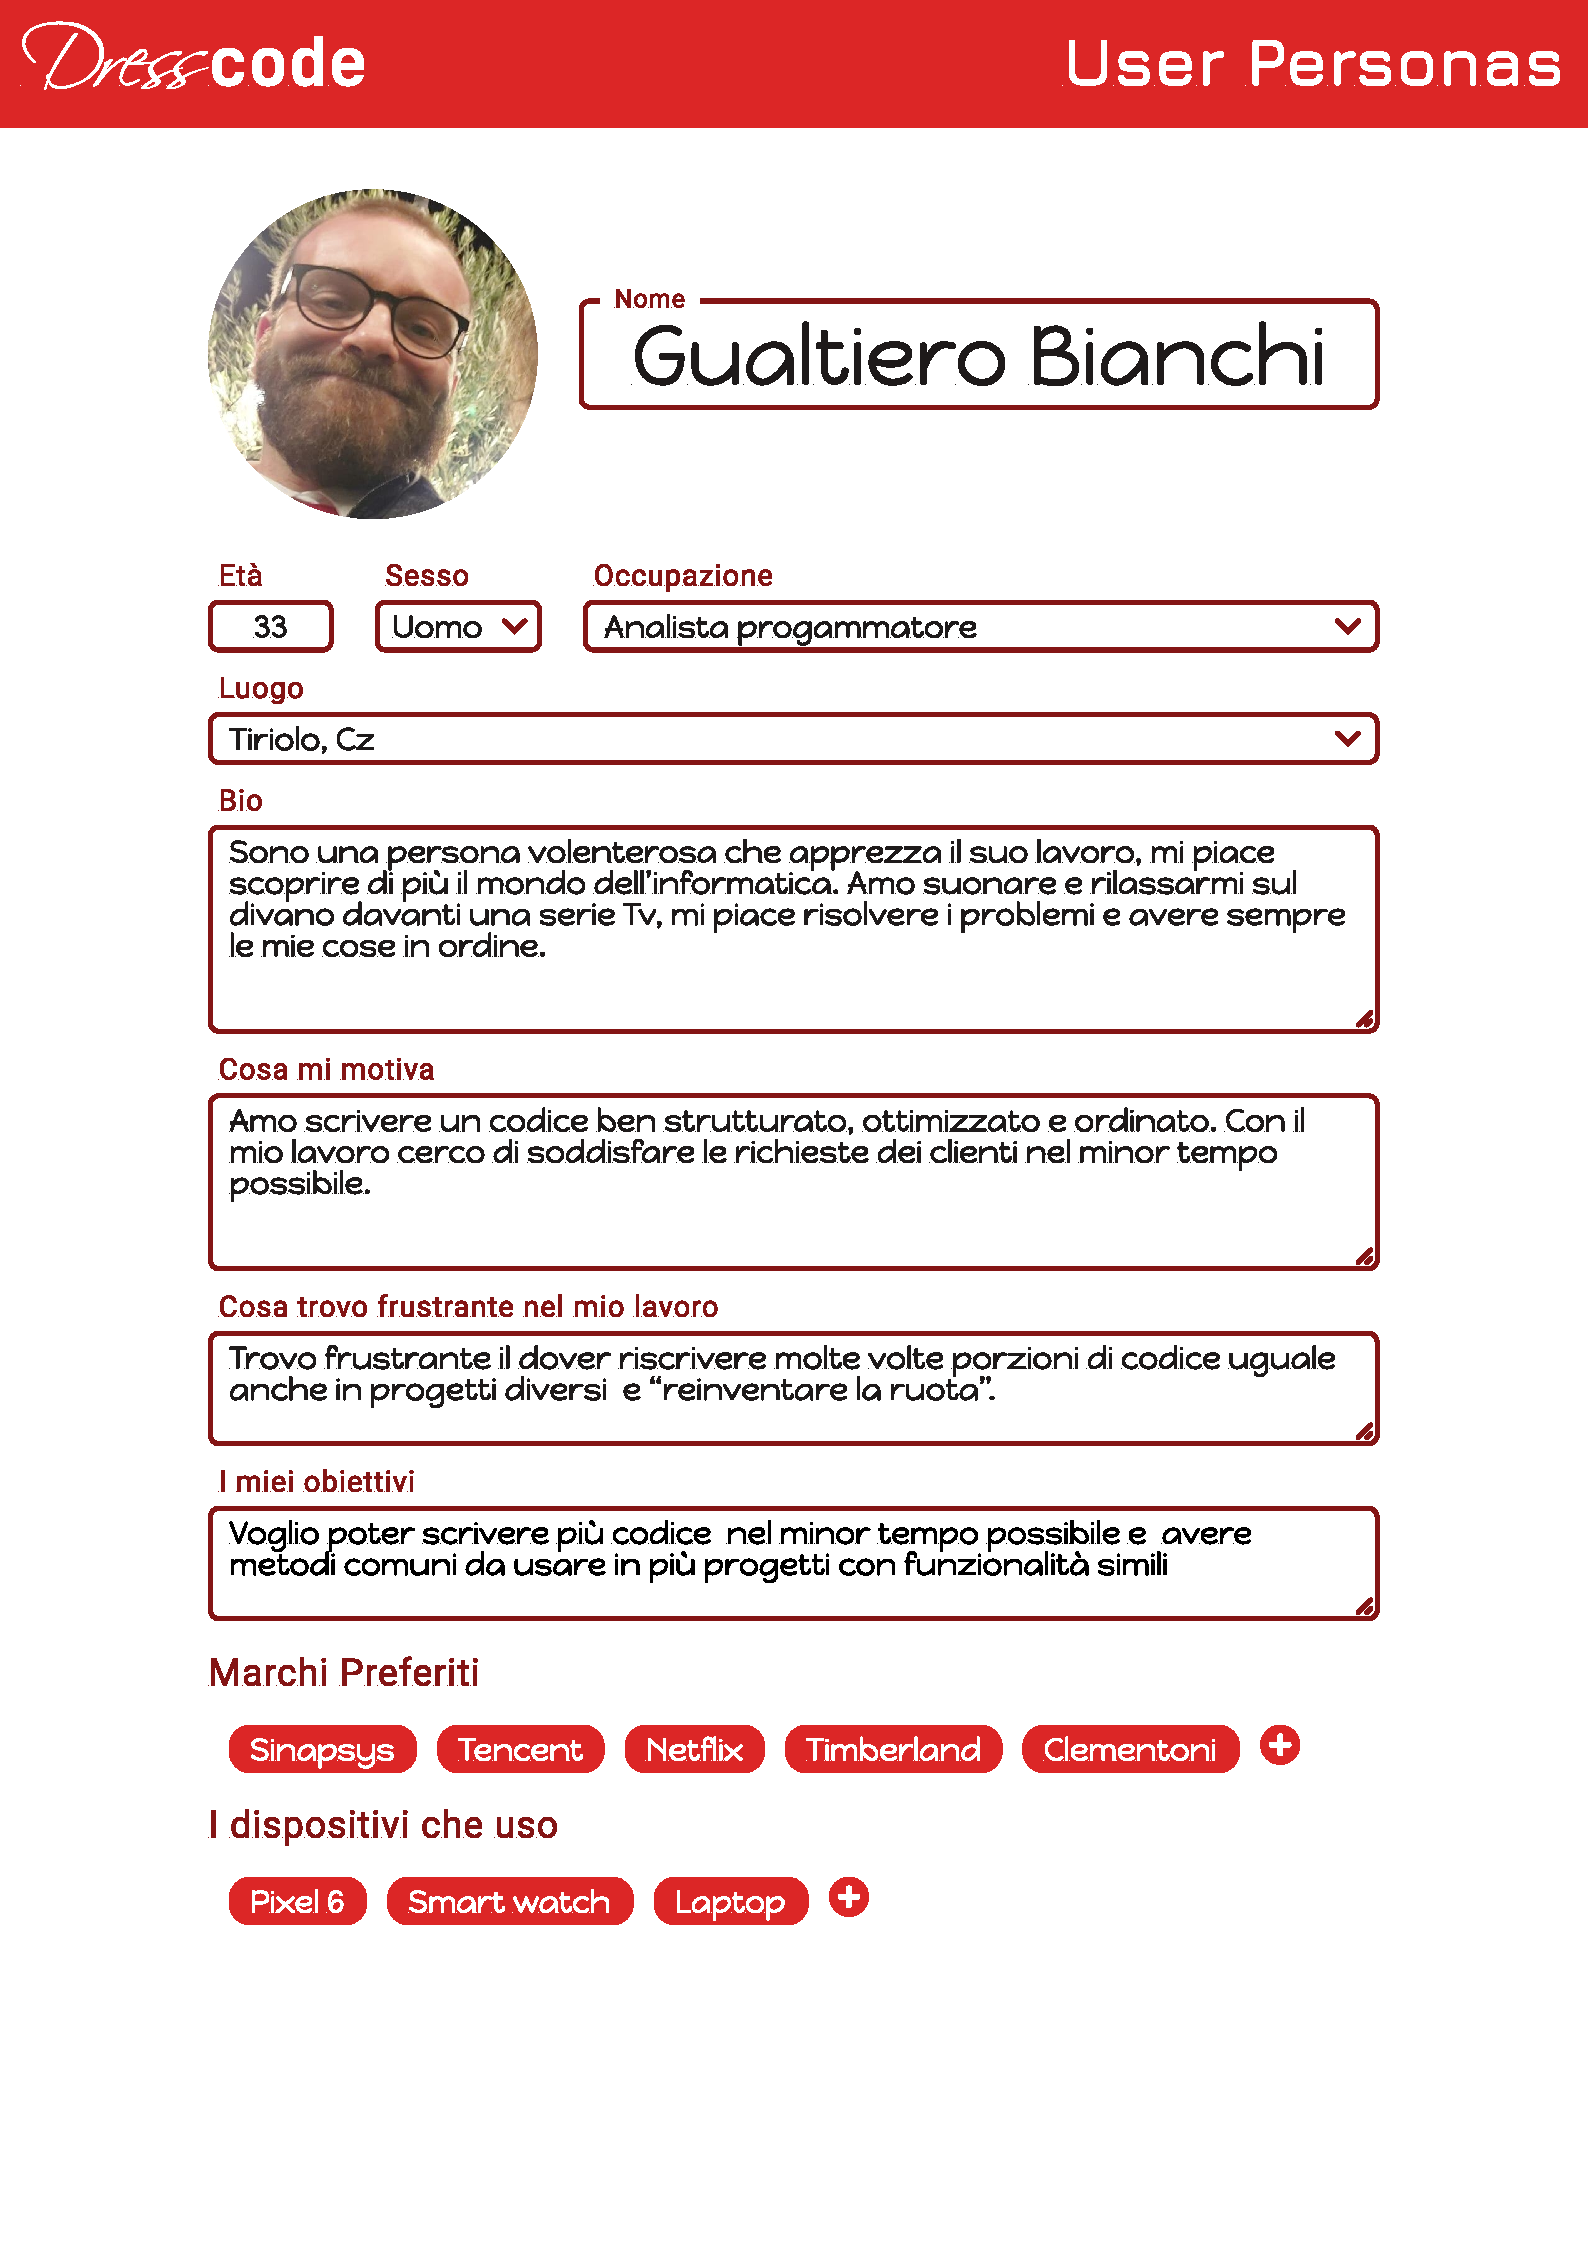
\includepdf[pages=-,pagecommand={}]{analisi degli utenti/personas_gualtiero_bianchi.pdf}